\section{Study: Using ReMap for a Graphic Design Task}
\label{sec:remap_study}
To gain an initial understanding of how people use multimodal search for help, we conducted a think-aloud lab study with thirteen participants. Participants re-created a given design in Canva (\href{https://canva.com}{\nolinkurl{canva.com}}) and used ReMap to search for help when necessary. Overall we found that despite some usability and implementation challenges, multimodal video search was helpful, allowing participants to stay focused on their task while simultaneously searching for help and navigating video resources. 

\subsection{Participants}
Thirteen participants were recruited from mailing lists and flyers at a university. 10/13 participants had at least some experience using voice assistants (\textit{e.g.}, Siri, Amazon Echo) (\textit{mean} = 2.3/5, 1 = never used, 5 = use every day). 6/15 participants had never used Canva before, and only one was very familiar with it (\textit{mean} = 1.8/5, 1 = never used, 5 = very familiar).

\subsection{Procedure}
Participants were given two images of an infographic design (\autoref{fig:remap_designs}) and were asked to choose one and re-create it as accurately as possible in Canva without using any of Canva's built-in templates. Participants were asked to use only ReMap (no web search) when they needed to search for help. Participants were given a brief tutorial on how to use ReMap, and were asked to try three example speech commands to ensure they understood how it worked. They were encouraged to use speech as much as possible, but also had the option to type their search queries into ReMap's search field and navigate videos using the mouse. Participants were asked to think out loud while they worked, and the experimenters captured audio and screen recordings. Participants were scheduled for 2-hour slots and were told to take as much time as they needed. Once they announced they were done (or if 1 hour and 45 minutes had passed), participants were asked a series of interview questions including prompts for Likert-scale responses to understand how they felt the task went, and whether they found ReMap helpful. Participants received a \$30 USD gift card for their time.

\begin{figure}[t!]
\centering
  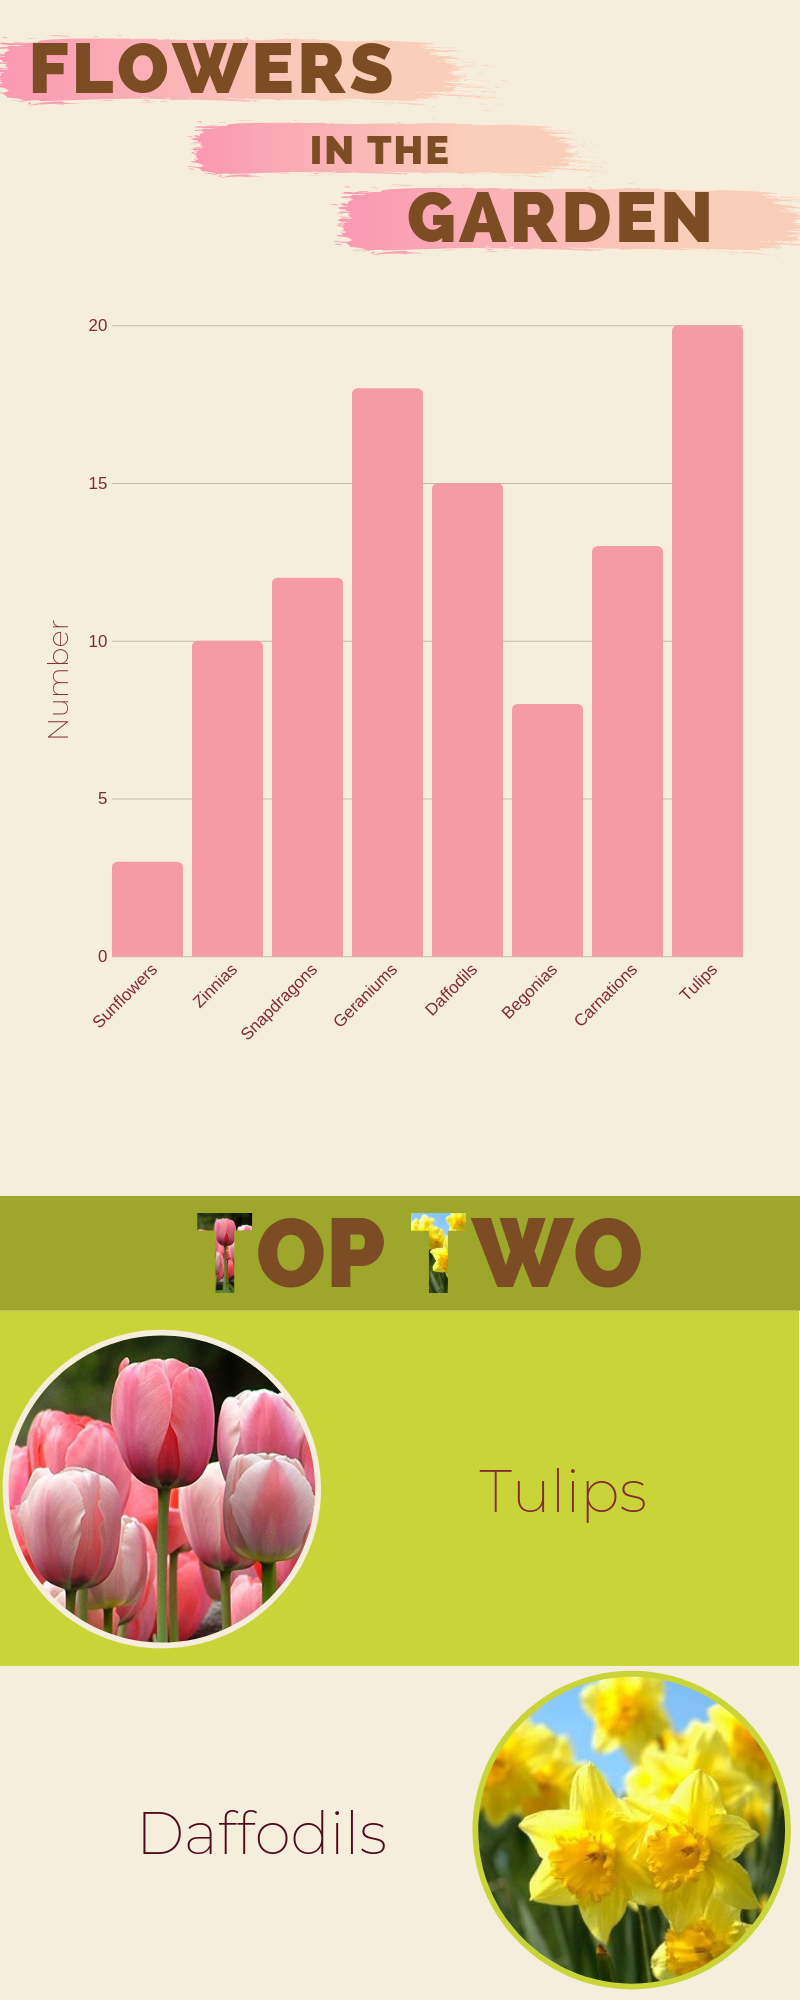
\includegraphics[width=0.3\textwidth]{remap/figures/designA.png}
  \hspace{0.2in}
  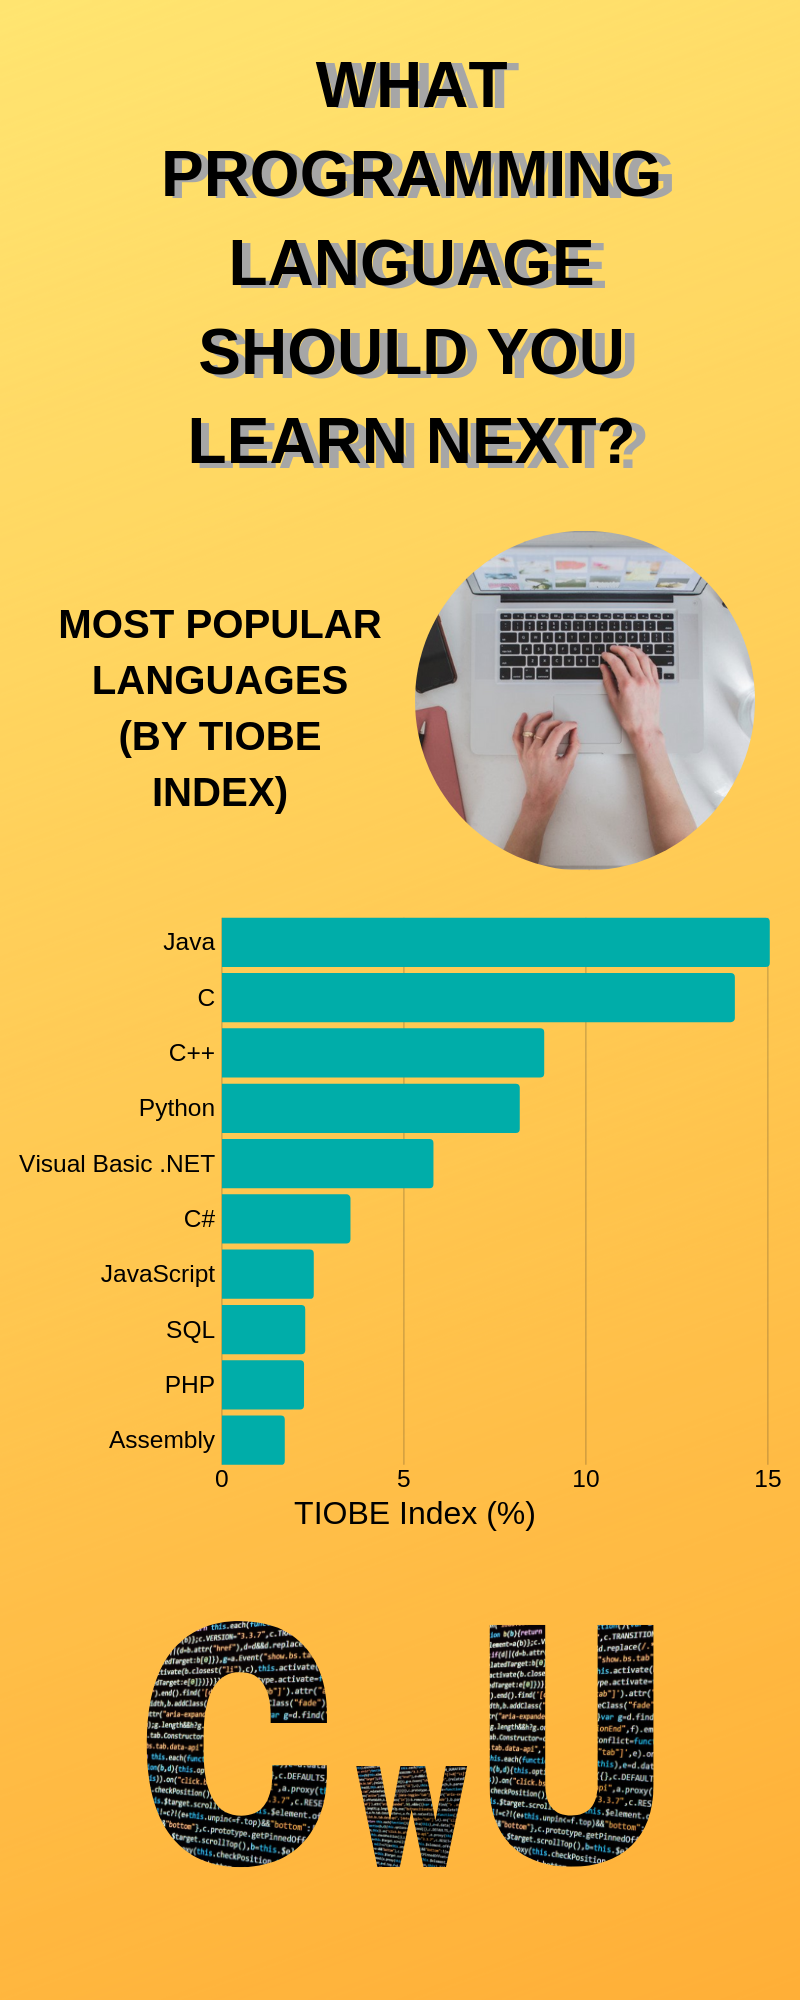
\includegraphics[width=0.3\textwidth]{remap/figures/designB.png}
  \caption{Study participants chose one of the above two infographic designs to re-create in Canva, using ReMap to search for help.}~\label{fig:remap_designs}
\end{figure}

Both infographics were designed to require several operations that are not straightforward in Canva, to increase the likelihood that participants would have to search for help. These included: cropping an image in a circle, masking an image with text, creating a bar chart given a spreadsheet of data, making a swish shape behind text (\autoref{fig:remap_designs} left only) and adding a shadow to text (\autoref{fig:remap_designs} right only).

ReMap's speech recognition requires a clear signal of the user's speech, mostly free of interference from sound output (\textit{i.e.} from videos) or background conversations. We have found commodity headsets to be sufficient, high-quality headsets to be optimal, and built-in laptop microphones insufficient. For the study, participants wore a high-quality headset.

\subsection{Results: Multimodal Search Enables Multitasking}
\subsubsection{Overview of Search Behaviour}
Participants issued a total of 118 intentional search queries, 111 of which used speech (\autoref{table:remap_results}). An additional 3 queries were issued by mistake (not realizing they had spoken the \textit{``search''} command) and an additional 7 were issued before the participant had finished speaking (because the Web Speech \textsc{api} detected a pause). One participant did not search at all (the same participant that rated their familiarity with Canva as 5/5); the rest issued between 3 and 17 queries each. 

\begin{table}[t!]
\centering
\caption{Summary of each participant’s usage of ReMap. ``\# speech commands'' includes all play, pause, and marker navigation commands. ``\# manual commands'' includes all plays, pauses, seeking along the timeline, and clicking on markers.}~\label{table:remap_results}
\resizebox{1\textwidth}{!}{
\begin{tabular}{lllllllll}
\textbf{} & \textbf{\begin{tabular}[c]{@{}l@{}}Total \#\\ intentional\\ searches\end{tabular}} & \textbf{\begin{tabular}[c]{@{}l@{}}\# accidental or\\ pre-emptive\\ searches\end{tabular}} & \textbf{\begin{tabular}[c]{@{}l@{}}\# intentional\\ speech\\ searches\end{tabular}} & \textbf{\begin{tabular}[c]{@{}l@{}}\# unique\\ videos\\ played\end{tabular}} & \textbf{\begin{tabular}[c]{@{}l@{}}\# speech\\ commands\end{tabular}} & \textbf{\begin{tabular}[c]{@{}l@{}}\# manual\\ commands\end{tabular}} & \textbf{\begin{tabular}[c]{@{}l@{}}\# deictic\\ references\end{tabular}} & \textbf{\begin{tabular}[c]{@{}l@{}}\# successful\\ deictic\\ resolutions\end{tabular}} \\ \hline
P1 & 17 & 1 & 17 & 13 & 41 & 3 & 5 & 1 \\
P2 & 5 & 0 & 5 & 6 & 2 & 93 & 1 & 0 \\
P3 & 13 & 3 & 13 & 7 & 20 & 23 & 10 & 1 \\
P4 & 4 & 0 & 4 & 5 & 14 & 19 & 0 & 0 \\
P5 & 0 & 0 & 0 & 0 & 0 & 0 & 0 & 0 \\
P6 & 8 & 1 & 8 & 5 & 17 & 2 & 0 & 0 \\
P7 & 7 & 1 & 7 & 6 & 24 & 10 & 0 & 0 \\
P8 & 3 & 1 & 3 & 2 & 4 & 1 & 0 & 0 \\
P9 & 8 & 1 & 6 & 6 & 0 & 49 & 0 & 0 \\
P10 & 16 & 0 & 13 & 5 & 10 & 5 & 3 & 0 \\
P11 & 10 & 1 & 10 & 11 & 9 & 51 & 1 & 1 \\
P12 & 11 & 0 & 11 & 4 & 8 & 16 & 1 & 1 \\
P13 & 16 & 1 & 14 & 7 & 18 & 0 & 3 & 2 \\
\textbf{Total} & \textbf{118} & \textbf{10} & \textbf{111} & \textbf{77} & \textbf{167} & \textbf{272} & \textbf{24} & \textbf{6}
\end{tabular}
}
\end{table}

61/118 queries (52\%) were new queries and 34/118 (29\%) were reformulations of previous queries (\textit{i.e.,} rephrasing a query to find better results). The rest were either attempts to fix a failed deictic resolution or fixing a transcription error. 55/118 queries (47\%) began with either the phrase \textit{``how to''} (42/118), or the phrase \textit{``how do I''} (13/118). 

8/111 speech queries included a speech recognition error. One participant tried to rephrase their query while speaking it, leading to long queries with some repetition (\textit{e.g.}, \textit{``resize this without aspect ratio without keeping aspect ratio''}). 6 of the 7 non-speech queries were a manual revision of a previous speech query (either error fixes or reformulations). 

\subsubsection{Deictic Resolution: Mostly Used for Canvas Elements}
7 of 13 participants used deictic references at least once, and 22\% (24/111) of spoken queries included a deictic reference. 23/24 deictic references referred to objects on the canvas (\textit{e.g.}, text boxes, images, and charts); the other referred to a button on the toolbar. This reinforces RePlay's study finding (\autoref{sec:replay_study}) that participants mostly made action-oriented queries, rather than queries about tools.

Unfortunately, only 25\% (6/24) of deictic references were successfully resolved to a name, mainly due to missing accessibility labels. For example, 10/18 unsuccessful deictic references were for charts, but charts in Canva do not have accessibility labels. We chose Canva for this study because it has more accessibility labels for canvas objects than most other creative applications; many do not label anything on the canvas at all. However, even Canva does not label all elements.

\subsubsection{Video Navigation Behaviour: Some Preferred Manual, Others Preferred Speech}
Participants watched a total of 77 videos (\textasciitilde6 videos per participant). In total, participants played videos by clicking on them 60 times, and by saying one of the \textit{``play''} commands 61 times. Participants paused manually 60 times, and via the \textit{``pause''} speech command 46 times. Participants manually seeked to points in the video by dragging on the timeline 124 times, by clicking timeline markers 28 times, and by saying the \textit{``next/previous/repeat marker''} commands 60 times. In general, most participants seemed to exhibit a preference for either speech commands or manual navigation of videos (\autoref{table:remap_results}). This highlights the importance of providing both options in a multimodal interface, especially as peoples' preferences and needs may change depending on their task or environment \cite{Reeves2004, LaViolaJr.2014}.

\subsubsection{Participant Feedback: Speech for Navigating Timeline Markers was Most Helpful}
As \autoref{fig:remap_boxplot} shows, participants generally found all four of ReMap's multimodal features moderately helpful. Based on our observations, most participants used the multimodal features to work and search or watch videos simultaneously. They confirmed this during the post-task interviews, with several participants explicitly mentioning multitasking as a benefit of ReMap's multimodal features. For example, one participant described how ReMap made them more efficient than their current strategies for help-seeking:

\begin{quote}
\textit{``When I'm designing graphics myself sometimes I get stuck, so I will have to stop everything and go to YouTube or Google to find it, but if I'm able to work while listening or ... watching it on the side, through voice, I think it will help with efficiency ... `cause at one point I was able to ... move the things around while listening for the things I need.''} --- P4
\end{quote}

\begin{figure}[t!]
\centering
  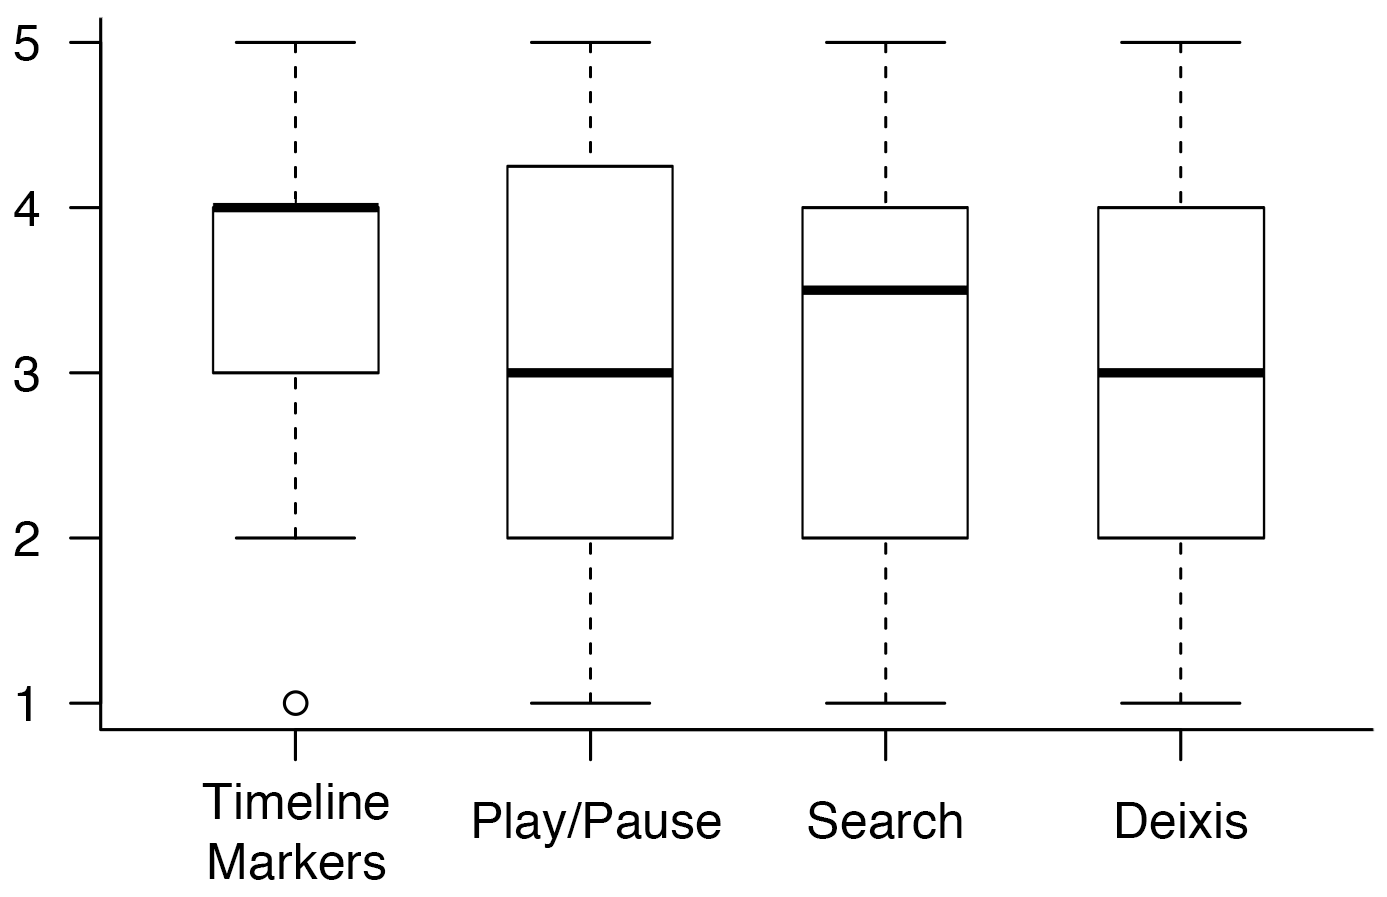
\includegraphics[width=0.7\textwidth]{remap/figures/boxplot.png}
  \caption{Distribution of participants' ratings of ReMap’s multimodal features. 1 = not helpful at all, 5 = very helpful. Bold lines represent median values, and boxes illustrate interquartile ranges. }~\label{fig:remap_boxplot}
\end{figure}

\textbf{Timeline markers:}
Navigating the timeline markers was rated as the most helpful multimodal feature on average, and was the most common answer participants gave when asked what their favorite feature of ReMap was. This is mainly because it supported participants in multitasking:

\begin{quote}
\textit{``I ... found it helpful because while it was switching I could multitask, and I could just tell it `hey, go to the next marker', and then I would try to do stuff on my own on the side until it plays.''} --- P6
\end{quote}

\begin{quote}
\textit{``If I couldn't use speech then I would have to ... actually click on the videos, but since I'm already working on this part of the screen, then [speech is] just more convenient.''} --- P7
\end{quote}

The markers themselves were useful (as the RePlay study (\autoref{sec:replay_study}) also showed) as they provided a shortcut to potentially relevant moments in the video. The speech commands for skipping between them made it easy for participants to back-up or fast-forward the video to a reasonable point. This is easier than having to specify a specific time interval to skip between, which Chang \textit{et al.} \cite{Chang2019} found can be difficult when following along with video tutorials. However, some participants did mention that they preferred using the mouse to hover over markers before selecting them, so they could see the caption previews (\autoref{fig:replay-green_markers}): \textit{``I don't really know what they are until I scroll over them''} (P11).

\textbf{Play/pause:}
Some participants found speech for playing and pausing videos to be helpful, as it allowed them to follow along with videos at their own pace, which prior work has also demonstrated the importance of \cite{Chang2019, Pongnumkul2011}.

\begin{quote}
\textit{``It's really helpful because if I hear the info I want and I'm kind of following along I can pause it, take the instructions, apply it, and then ... continue watching ... without having to stop the fluidity of work.''} --- P8
\end{quote}
\begin{quote}
\textit{``It was nice to be able to keep track of the video in the background while also starting to think through the next thing and having my focus on the other window.''} --- P13
\end{quote}

Other participants preferred using the mouse to play and pause videos as they felt it was just as fast or easy, and didn't require them to remember the correct wording of the commands.

\textbf{Speaking queries:}
Many participants found it helpful to speak their query out loud rather than type it, as it allowed them to stay focused on the task in Canva while searching. Some also said that it was easier or faster than typing. However, some other participants found it more difficult to speak their query, as they didn't always know exactly what to say when they started, and they were not used to speaking out loud to search. As P13 described, \textit{``I had a lot of trouble getting my queries totally straight or thought out in my head before starting to speak them.''} One difficulty sometimes encountered with ReMap's implementation was that it would cut off a participant's query and issue the search before they were done speaking, often because they paused slightly while thinking of what to say. This happened 7 times and was due to the Web Speech \textsc{api} prematurely detecting the end of a phrase. As one participant described, it made them feel rushed to finish speaking:

\begin{quote}
\textit{``It kept rushing me to think about what I wanted to search for ... Usually when I search by typing, I type out half of what I want and then think about ... what to type for the rest, whereas here as soon as i said `how to add' I had to immediately know what I was searching.''} --- P6
\end{quote}

\textbf{Deixis:}
The 7 participants who attempted using deixis in their queries mostly found it helpful, although many noted that it needed some improvement to be useful, as it often failed to recognize the referenced element. When it did succeed, it helped participants include words they didn't know in their queries and was often easier and faster than saying or typing the words explicitly. However, it is likely most helpful in cases where users do not know the terminology, and Canva's interface has a relatively straightforward vocabulary. Deictic resolution might be used more frequently in software that has a more complex interface. For example, P1, who rated their prior experience with Canva as 1.75/5, said \textit{``it might be more helpful for things that you don't know the exact terminology for, but I think I knew some of the terminology so just saying it felt faster.''}

Two participants also pointed out that their eyes naturally went to the search field where their query was appearing while they spoke it, which made it difficult to look at Canva to reference elements: \textit{``even though I was trying to click here I was focusing on [the search field]''} (P9).

\textbf{Overall:}
Finally, when asked if participants could see themselves using ReMap in their daily lives, 9 participants said yes (3 saying for certain tasks only, and 2 saying if the technology improved first). The 4 participants who said no shared reservations about using speech in public or around people, and some said they simply prefer typing.
